\section{Bayesian single parameter models}

Last class we saw our first single parameter model for Binomial data.

\begin{table}[ht]
\centering
\begin{tabular}{@{}llll@{}}
\toprule
       & Pass & Fail & Total \\ \midrule
Whites & 206  & 53   & 259   \\
Blacks & 26   & 22   & 48    \\ \bottomrule
\end{tabular}
\caption{Connecticut vs. Teal: 1982 Supreme Court Case}
\end{table}

We have

\begin{align*}
    y_B \sim& \text{Binomial}(n, \theta_B)\\
    \theta_B \sim& \text{Beta}(\alpha, \beta),
\end{align*}

as discussed in the last section, the conjugate prior that gives us a Beat prior distribution 

\[
\theta \sim \text{Beta}(y_B + \alpha, n_B + \beta)
\]

The difficult part it the ``noninformative'' options for $\alpha$ and $\beta$.

\begin{itemize}
    \item $\alpha = \beta = 0$: improper flat prior
    \item $\alpha = \beta = 1$: uniform (0, 1) prior
    \item $\alpha = \beta = \frac{1}{2}$: Jeffery's prior
    \item $\alpha = \beta = \frac{1}{3}$: Neutral's prior
\end{itemize}

\subsection{R Example}
\begin{enumerate}
    \item Show basic effect of Bayes rule updating. Compare $\theta_B \sim \text{Unif}(0, 1)$ to $\theta_B | y_B \sim \text{Beta}(27, 33)$.
    \begin{figure}[H]
    	\centering
    	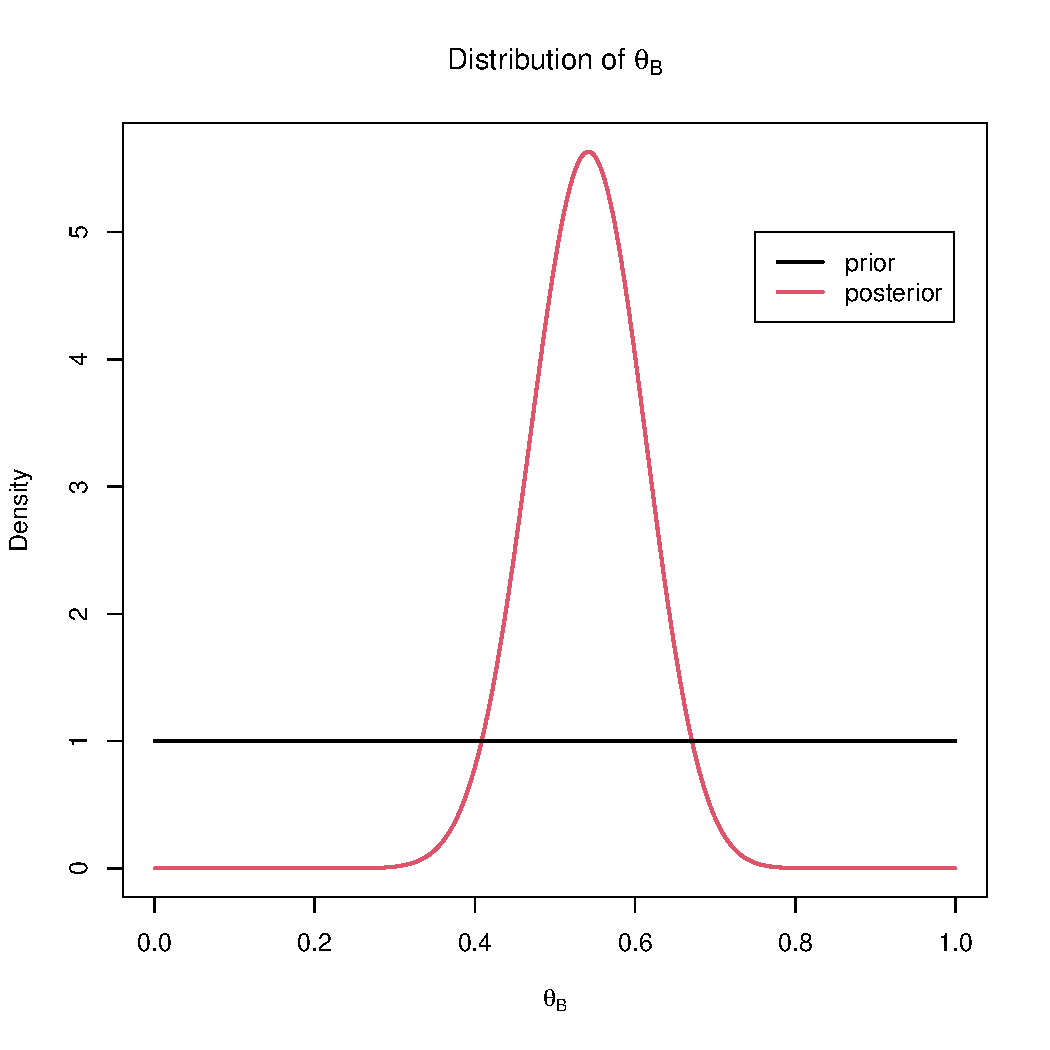
\includegraphics[width=0.6\textwidth]{../R/fig/fig1.pdf}
    \end{figure}
    \item Compare second different conjugate prior for Binomial model on both a small synthetic dataset and the Connecticut vs. Teal date.
    \begin{figure}[H]
    	\centering
    	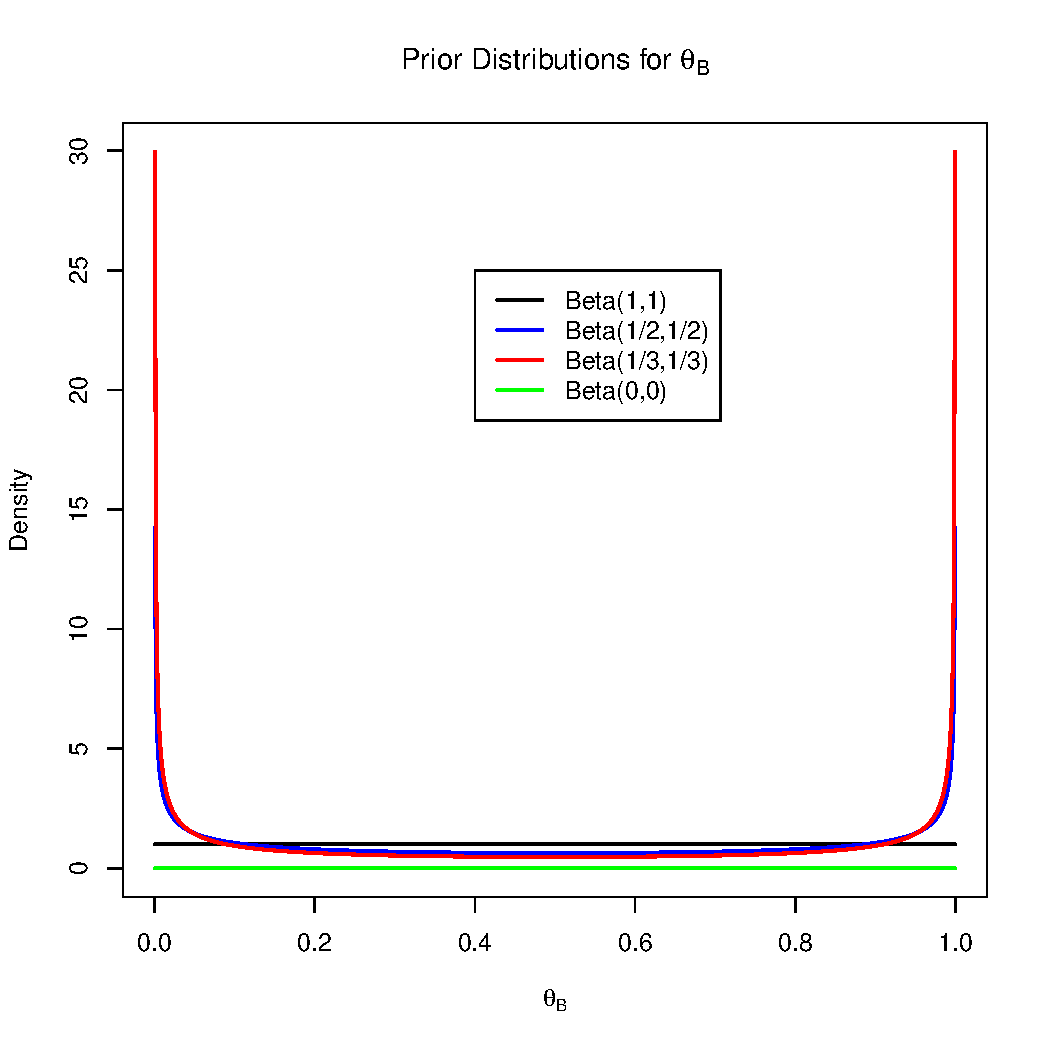
\includegraphics[width=0.6\textwidth]{../R/fig/fig2.pdf}
    \end{figure}
    \begin{figure}[H]
    	\centering
    	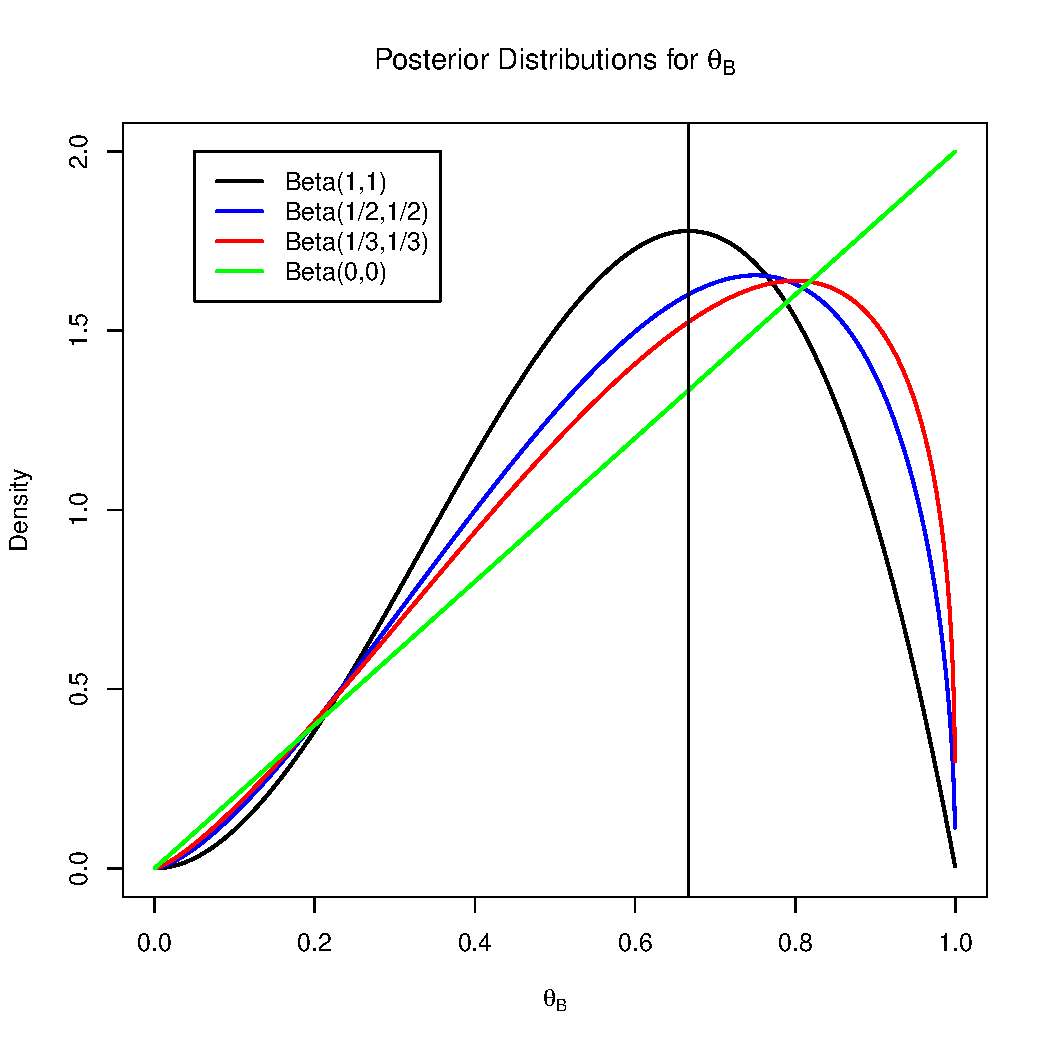
\includegraphics[width=0.6\textwidth]{../R/fig/fig3.pdf}
    \end{figure}
    \item Show plot comparing $\theta_B \sim \text{Beta}(27, 23)$ to $\theta_W| y_w \sim \text{Beta}(207, 54)$. Clearly, $\theta_W$ is shifted to $\theta_B$.
    \begin{figure}[H]
    	\centering
    	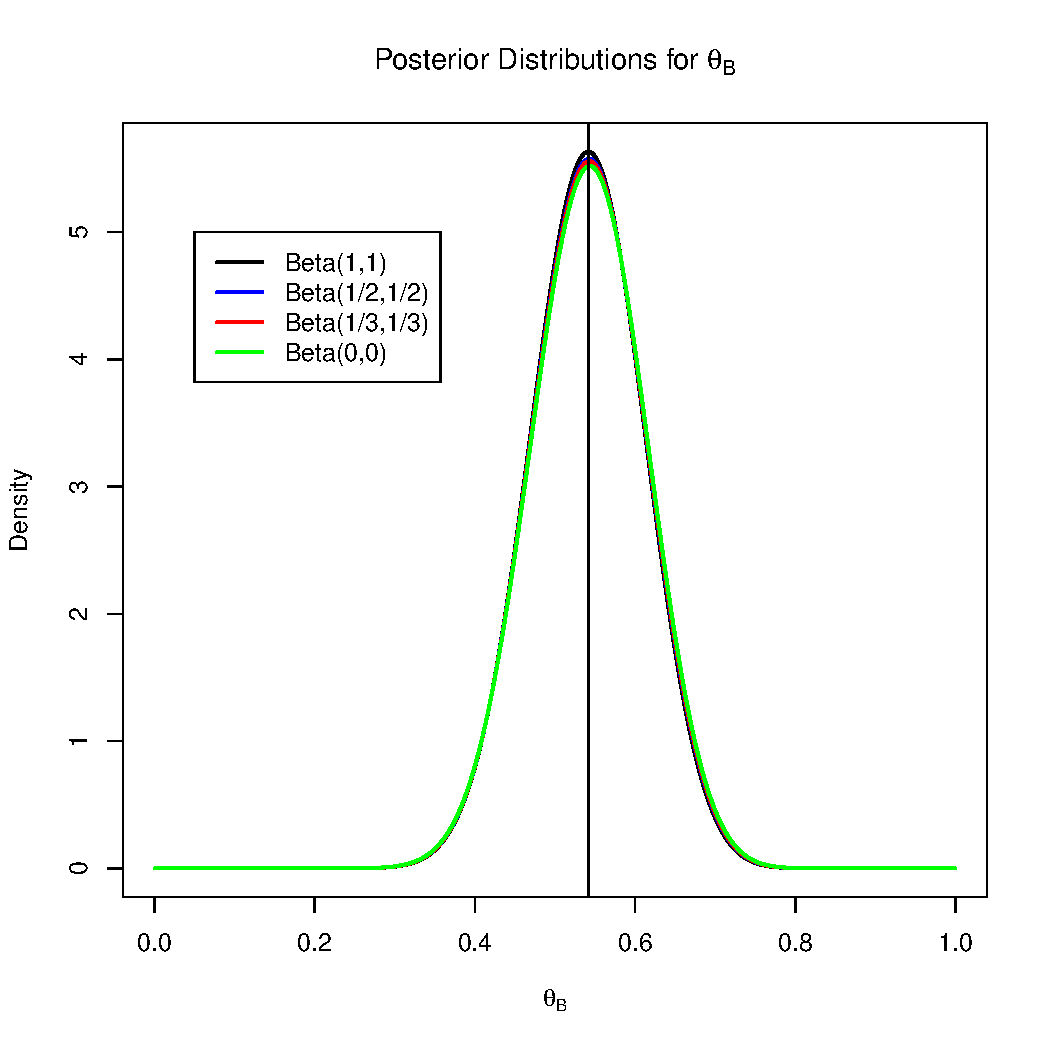
\includegraphics[width=0.6\textwidth]{../R/fig/fig4.pdf}
    \end{figure}
\end{enumerate}

What we really want is $\p(\theta_W > \theta_B | y)$.

\[
\p(\theta_w > \theta_B | y_W, y_B) = \iint_{\theta_W > \theta_B} \p(\theta_w, \theta_B| y_w, y_B) \diff \theta_w \diff \theta_B.
\]

If we assume $\p(\theta_w, \theta_B) = \p(\theta_w) \p(\theta_B)$ and $y_B|\theta_B \indep y_w| \theta_B$, then

\begin{align*}
    \p(\theta_w, \theta_B | y_w, y_B) 
    =& \p(y_w| \theta_w)\p(\theta_w) \cdot \p(y_B| \theta_B) \cdot \p(\theta_B)\\
    =& \p(\theta_w| y_w) \cdot \p(\theta_B| y_B)
\end{align*}

So how do we do this integral with these posterior distribution?

If you are really good at calculus, maybe you can do that integral analytically. But it is much easier to calculate the integral by simulation. The steps are as follows. 

\begin{enumerate}[(a)]
    \item Sample $N$ values of $\theta_B|y_B \sim \text{Beta}(27, 23)$.
    \item Sample $N$ values of $\theta_w|y_w \sim \text{Beta}(207, 54)$.
    \item Pair up values from (a) and (b) and calculate proportion when $\theta_W > \theta_B$.
\end{enumerate}

From computer calculation, $\p(\theta_w > \theta_B| y) > 0.9999$.

We can do prediction with the posterior prediction distribution.
\begin{itemize}
    \item (e.g.) How many predicted successes in next 100 blacks?
    We have 
    \[
    \p(y^*| y_B) = \int \p(y^*_B | \theta_B) \cdot \p(\theta_B| y_B) \diff \theta_B,
    \]
    where
    \begin{itemize}
        \item $\p(y^*_B | \theta_B)$ is the uncertainty in new data, $\text{Bin}(100, \theta_B)$.
        \item $\p(\theta_B| y_B)$ is the uncertainty in model parameters, $\text{Beta}(27, 23)$.
    \end{itemize}
    Again, easiest to do this integral by simulation as follows.
    \begin{enumerate}[(a)]
        \item Draw $N$ values of $\theta_B|y \sim \text{Beta}(27, 23)$.
        \item For each $\theta_B$ from (a), draw $y^*_B \sim \text{Binomial}(100, \theta_B)$.
    \end{enumerate}
    Sample $y_B^*$ gives us an approximation of $\p(y_B^*|y_B)$.
\end{itemize}

\subsection{Compare with classical approach to prediction}

Parametric bootstrap: simulate $y^*_B \sim \p(y_B^*| \theta_B)$. Accounts for uncertainty is new data but not in underlying parameter. 

\subsection{Poisson Data}
Poisson Data: count data when the number of approximation is not known. $Y=0, 1, 2, \cdots$.

\[
y_i \sim \text{Poisson}(\theta), ~i=1, \cdots, n
\]

The likelihood is 
\[
\p(\vec{y}|\theta) 
= \prod_{i=1}^n \frac{\theta^{y_i} e^{-\theta}}{y_i!} 
= \frac{\theta^{\sum y_i} e^{-n\theta}}{\prod_{i=1}^n y!}
\approx \theta^{\sum y_i} e^{-n \theta}
\]

Is there a conjugate prior for this likelihood? Yes! $\theta \sim \text{Gamma}(\alpha, \beta)$.
\[
\p(\theta) = \frac{\beta^{\alpha}}{\prod(\alpha)} \theta^{\alpha-1} e^{\beta \theta} \approx \theta^{\alpha-1} e^{-\beta \theta},
\]
which gives a prosterior of 

\[
\p(\theta|y) \approx \p(y|\theta) \cdot \p(\theta) \approx \theta^{\sum y_i + \alpha - 1} e^{-n(n+\beta)}
\]

So 
\[
\theta|y \sim \text{Gamma}(\sum y_i + \alpha, n + \beta)
\]

So we can interpret a $\theta \sim \text{Gamma}(\alpha, \beta)$ prior as adding $\beta$ prior observations with a total count of $\alpha$.

Posterior is a compromise between $\hat \theta_\MLE$ and $\E(\theta) = \frac{\alpha}{\beta}$.

\subsubsection{Jefferys Prior for Poisson Model}
\begin{align*}
    \p(\vec{y}| \theta) \approx& ~\theta^{\sum y_i} e^{-n\theta}\\
    l(y|\theta) =& ~k + \sum y_i \log \theta - n \theta\\
    \pdv{l}{\theta} =&~ \frac{\sum y_i}{\theta} - n\\
    \pdv[2]{l}{\theta} =&~ \frac{-\sum y_i}{\theta^2}\\
    -\E[\pdv[2]{l}{\theta}] =&~ \frac{n\theta}{\theta^2} = \frac{n}{\theta}
\end{align*}

Therefore, Jeffery's Prior is $\p(\theta) \approx \theta^{-1/2} \iff \theta \sim \text{Gamma}(\alpha=\frac{1}{2}, \beta=0)$.

\subsubsection{R Example: Poisson with Planet Data}

Let's talk about one more single parameter model, Normal Data with known variance. This is not a particularly useful model but can give us some additional insight about Prior design.

\begin{align*}
    y_i 
    \sim&~ N(\mu, \sigma^2), ~\text{$\sigma$ is known}.\\
    \p(\vec{y}| \mu) 
    =&~ \prod_{i=1}^n \frac{1}{\sqrt{2\pi \sigma^2}} e^{-\frac{1}{2\sigma^2} (y_i - \mu)^2} \\
    \approx&~ e^{-\frac{1}{2\sigma^2} \sum_{i=1}^{n} (y_i - \mu)^2}
\end{align*}

Is there a conjugate prior to this likelihood? Yes! The normal is conjugate for itself!
\begin{align*}
    \mu \sim N(\mu_0, \tau^2), ~\p(\mu) \approx e^{-\frac{1}{2\tau^2} (y_i - \mu)^2}
\end{align*}

The posterior distribution is

\[
\p(\mu | y) \approx e^{-\frac{1}{2\sigma^2} \sum (y_i - \mu)^2 - \frac{1}{2\sigma^2} (\mu - \mu_0)^2}
\]

Therefore, we have

\[
\mu|y \sim \text{Norm}(\frac{\frac{n}{\sigma^2} \bar{y} + \frac{1}{\tau^2} \mu_0}{\frac{n}{\sigma^2} + \frac{1}{\tau^2}}, \frac{1}{\frac{\mu}{\sigma^2} + \frac{1}{\tau^2}})
\]

Posterior mean is again a compromise between $\hat \mu_\MLE = \bar{y}$ and prior mean $\mu_0$. The weights on this compromise are controlled by data variance $\sigma^2$, prior variance $\tau^2$ and sample size $n$. As $n \rightarrow \infty$, $\bar{y}$ dominates regradless of the prior. If $n$ is small, then we can still make the prior non informative by taking $\tau^2 \rightarrow \infty$.

Note that $\tau^2 \rightarrow \infty \Rightarrow \p(\mu) \approx 1$ flat prior are with real line. This prior is improper but still leads to a proper posterior, as long as $\sigma^2 > 0$ and $n > 0$.

What about Jeffery's Prior?

\begin{align*}
    \l(y| \mu) =& k - \frac{1}{2\sigma} \sum(y_i - \mu)^2\\
    \pdv{l}{\mu} =& \frac{1}{\sigma} \sum(y_i - \mu)\\
    \pdv[2]{l}{\mu} =& - \frac{n}{\sigma}
\end{align*}

$J(\mu) = \frac{n}{\sigma^2}$ which is a constant w.r.t $\mu$ so flat prior $\p(\mu) \approx 1$ is also the Jeffery's Prior in this case.

With the flat prior $\p(\mu) \approx 1$, posterior becomes
\[
\mu | y \sim N(\bar(y), \sigma^2/n),
\]
which is familiar as the sampling distribution from classical statistics.

The posterior predictive distribution for this simple normal model is also interesting:

\[
\p(y^*| y) = \int_{-\infty}^{\infty} \p(y^*| \mu) \cdot \p(\mu| \vec{y}) \diff \mu 
\]

\begin{itemize}
    \item $\p(y^*| \mu)$ is $y^* \sim N(\mu, \sigma^*)$
    \item $\p(\mu| \vec{y})$ is $\mu|y \sim N()$
\end{itemize}

Since normal is conjugate for itself, we know the resulting distribution will also be normal.

\[
y^*|y \sim \text{Normal}(
\frac{\frac{n}{\sigma^2} \bar{y} + \frac{1}{\tau^2} \mu_0}{ \frac{n}{\sigma^2} + \frac{1}{\tau^2}},
\sigma^2 + \frac{1}{\frac{n}{\sigma^2} + \frac{1}{\tau^2}})
\]

Now let's leverage our normal model to be more useful case where we have both unknown mean and variance.
\[
y_i \sim N(\mu, \sigma^2), \theta = (\mu, \sigma^2)
\]

This is our first multiparameter model.

Likelihood
\begin{align*}
    \p(\vec{y}| \theta) 
    =& (\frac{1}{\sqrt{2\pi}\sigma})^n \exp(-\frac{1}{2\sigma^2} \sum_{i=1}^n(y_i - \mu)^2)\\
    \approx& (\sigma^2)^{-n/2} \exp(-\frac{1}{2\sigma^2} \sum_{i=1}^n(y_i - \mu)^2)
\end{align*}

We need to construct a joint prior distribution for $\vec{\theta} = (\mu, \sigma^2)$. We will examine three prior s for this model
\begin{itemize}
    \item Conjugate
    \item Non informative
    \item Semi conjugate
\end{itemize}

